\documentclass[a4paper,12pt]{book}
\usepackage[utf8]{inputenc}
\title{}
\author{Rachel Morris}
\date{\today}

\usepackage{rachwidgets}
\usepackage{fancyhdr}
\usepackage{lastpage}
\usepackage{dirtree}
\usepackage{boxedminipage}

\newcommand{\laClass}{CS 211\ }
\newcommand{\laSemester}{Fall 2017\ }
\newcommand{\laChName}{Hamiltonian Cycles and the TSP\ }
\newcounter{question}

\setcounter{chapter}{7}
\setcounter{section}{6}
\newcommand{\laChapter}{7.7 \laChName}

\pagestyle{fancy}
\fancyhf{}
\lhead{\laClass Exercise, \laSemester}
\chead{}
\rhead{Ch \laChapter}
\rfoot{\thepage\ of \pageref{LastPage}}
\lfoot{\scriptsize Compiled by Rachel Morris, last updated \today}

\renewcommand{\headrulewidth}{2pt}
\renewcommand{\footrulewidth}{1pt}

\begin{document}

    %\toggletrue{answerkey}
    \togglefalse{answerkey}

    \section{\laChName}
    
    \notonkey{

    %- Team Info ------------------------------------------------------%

    Please write down all people in your team. ~\\

    % table %
    \begin{tabular}{ p{6cm} p{6cm} }
        1. & 2. \\ \\
        3. & 4.
    \end{tabular} ~\\
    % table %
    
    \hrulefill
    
    }{}


    \subsection{Hamiltonian Cycles}

    \notonkey{
        \begin{intro}{Review \& Hamiltonian cycle}
            \paragraph{Walk:} A series of alternating nodes and edges traversing between adjacent nodes.

            \paragraph{Path:} A walk with no repeated vertices.

            \paragraph{Circuit:} A closed trail.
            
            \paragraph{Trail:} A walk with no repeated edges.
            
            \paragraph{Cycle:} A nontrivial circuit where the only repeated node is the first/last one.
            
            \paragraph{Hamiltonial cycle:} A Hamiltonian cycle in $G$ is a cycle
            that uses every node of $G$. The graph $G$ is called Hamiltonian
            if it contains a Hamiltonian cycle.

            \paragraph{Eulerian trail or circuit:} A trail or circuit where every edge is traversed
            \footnote{Discrete Mathematics, Ensley and Crawley}
        \end{intro}
        
        \newpage
    }{}

    
% -------------------------------------------------------------%
% - QUESTION --------------------------------------------------%
% -------------------------------------------------------------%
\stepcounter{question}
\begin{question}{\thequestion}{1}
    For the following graph, trace out a Hamiltonian cycle.
    You can use the Hamiltonian Cycle visualization from \\
    https://rachels-courses.github.io/Visualizations/ to practice.

    \begin{center}
        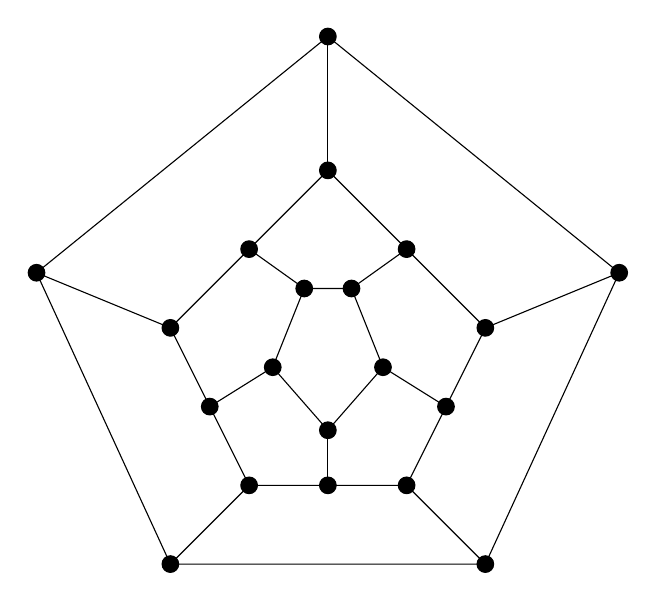
\begin{tikzpicture}
            \filldraw (-2,0) circle (3pt);
            \filldraw (2,0) circle (3pt);
            \filldraw (-3.7,3.7) circle (3pt);
            \filldraw (3.7,3.7) circle (3pt);
            \filldraw (0,6.7) circle (3pt);
            \draw (-2,0) -- (2,0) -- (3.7,3.7) -- (0,6.7) -- (-3.7,3.7) -- (-2,0);

            \filldraw (-1,1) circle (3pt);
            \filldraw (0,1) circle (3pt);
            \filldraw (1,1) circle (3pt);
            \filldraw (1.5,2) circle (3pt);
            \filldraw (-1.5,2) circle (3pt);
            \filldraw (-2,3) circle (3pt);
            \filldraw (2,3) circle (3pt);
            \filldraw (-1,4) circle (3pt);
            \filldraw (1,4) circle (3pt);
            \filldraw (0,5) circle (3pt);
            \draw (-1,1) -- (0,1) -- (1,1) -- (1.5,2) -- (2,3) -- (1,4) -- (0,5)
                -- (-1,4) -- (-2,3) -- (-1.5,2) -- (-1,1);
            \draw (-1,1) -- (-2,0);
            \draw (1,1) -- (2,0);
            \draw (-2,3) -- (-3.7,3.7);
            \draw (2,3) -- (3.7,3.7);
            \draw (0,5) -- (0,6.7);

            \filldraw (0,1.7) circle (3pt);
            \filldraw (-0.7,2.5) circle (3pt);
            \filldraw (0.7,2.5) circle (3pt);
            \filldraw (0.3,3.5) circle (3pt);
            \filldraw (-0.3,3.5) circle (3pt);
            \draw (0,1.7) -- (-0.7,2.5) -- (-0.3,3.5) -- (0.3,3.5)
                -- (0.7,2.5) -- (0,1.7);
            \draw (0,1.7) -- (0,1);
            \draw (-0.7, 2.5) -- (-1.5,2);
            \draw (0.7, 2.5) -- (1.5,2);
            \draw (0.3,3.5) -- (1,4);
            \draw (-0.3,3.5) -- (-1,4);
        \end{tikzpicture}
    \end{center}
\end{question}

    \hrulefill

    \notonkey{
        \begin{intro}{Hamiltonian puzzle and Hamiltonial path problem}
            
            The Hamiltonian puzzle involves finding a Hamiltonian cycle
            in the edge graph of a dodecahedron.

            Determining whether Hamiltonian cycles exist in graphs is
            the Hamiltonian path problem, which is NP-complete.
            \footnote{From https://en.wikipedia.org/wiki/Hamiltonian\_cycle}
            ~\\

            NP complete means ``nondeterministic polynomial time'', where
            a solution to an NP-complete problem can be verified quickly,
            but there is no known efficient way to locate a solution
            in the first place.
            \footnote{From https://en.wikipedia.org/wiki/NP-complete\_problem}
        \end{intro}

        \newpage
    }{}

    \subsection{Travelling Salesperson}

    \notonkey{
        \begin{intro}{\ }
            The ``TSP'' is another type of problem that asks the following:
            \footnote{From https://en.wikipedia.org/wiki/Travelling\_salesperson\_problem}
            
            \begin{center}
                ``Given a list of cities and the distances between each pair of cities, what is the shortest possible route that visits each city exactly once and returns to the origin city?''
            \end{center}
        \end{intro}
    }{}

    Go to https://rachels-courses.github.io/Visualizations/ and use the
    \textbf{Travelling Salesperson} visualization to help you work on this part.
    
    \begin{center}
        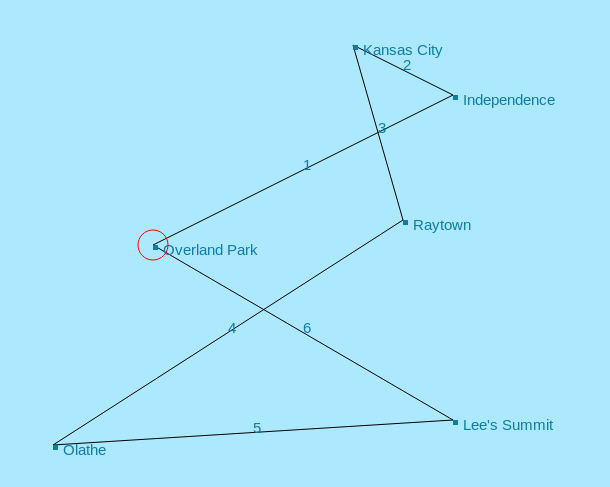
\includegraphics[width=8cm]{images/7-7-salesperson.png}
    \end{center}

    Click on any node to begin the path. Click on subsequent nodes to add
    an edge between the nodes. The program records the distance (in pixels)
    at the bottom of the screen.

\hrulefill

% -------------------------------------------------------------%
% - QUESTION --------------------------------------------------%
% -------------------------------------------------------------%
\stepcounter{question}
\begin{question}{\thequestion}{1}

    If we have 6 total cities to visit, with the last city being visited twice,
    how many possible ways can we visit all cities?

    ~\\
    \begin{center}
        \begin{tabular}{c c c c c c c}
            \fitb & \fitb & \fitb & \fitb & \fitb & \fitb & \fitb
            \\
            1 (start) & 5 & 4 & 3 & 2 & 1 & 1 (end)
            %\\
            %OP & OL & LS & RT & IN & KC & OP
        \end{tabular}
    \end{center}

    \solution{ $1 \cdot P(5,5) \cdot 1 = 120 $}
    
\end{question}

    \newpage

% -------------------------------------------------------------%
% - QUESTION --------------------------------------------------%
% -------------------------------------------------------------%
\stepcounter{question}
\begin{question}{\thequestion}{1}
    
    Come up with three different \textbf{cycles}, where all nodes
    are visited exactly once - except the starting point, which is visited
    first and last. Record the distances found for each. The starting
    city should be Overland Park.

    ~\\
    \begin{tabular}{ | l | p{9cm} | l |}
        \hline
        \# & Walk & Total distance
        \\ \hline
        1. & OP $\to$ Olathe $\to$ Lee's Summit $\to$ Raytown $\to$ Independence $\to$ Kansas City $\to$ Overland Park & 1360
        \\ \hline
    \end{tabular}

    \vspace{10cm}
    What kind of method (if any) did you use to try to find a shortest path?

\end{question}

\newpage

%According to the ``As The Crow Flies'' Distance Calculator at \\
%http://tjpeiffer.com/crowflies.html,
%the distance between each of the cities given, in miles, in the visualization are:

%\begin{center}
    %\begin{tabular}{r | c c c c c c}
                %& Indep.    & K.C.      & L.S.  & Olathe    & O.P.      & Raytown
        %\\ \hline
        %Indep.  & 0         & 9         & 13    & 26        & 16        & 6
        %\\
        %K.C.    & 9         & 0         & 17    & 20        & 10        & 9
        %\\
        %L.S.    & 13        & 17        & 0     & 24        & 16        & 8
        %\\
        %Olathe  & 26        & 20        & 24    & 0         & 11        & 21
        %\\
        %O.P.    & 16        & 10        & 16    & 11        & 0         & 11
        %\\
        %Raytown & 6         & 9         & 8     & 21        & 11        & 0
    %\end{tabular}
%\end{center}


% -------------------------------------------------------------%
% - QUESTION --------------------------------------------------%
% -------------------------------------------------------------%
\stepcounter{question}
\begin{question}{\thequestion}{1}
    Fill out the following table to record the distance between any two cities,
    given by the visualization.
    ~\\~\\
    \Large 
    \begin{tabular}{r | c | c | c | c | c | c}
                & Indep.    & K.C.      & L.S.  & Olathe    & O.P.      & Raytown
        \\ \hline
        Indep.  & 0         &          &     &         &         & 
        \\ \hline
        K.C.    &          & 0         &     &         &         & 
        \\ \hline
        L.S.    &         &         & 0     &         &        & 
        \\ \hline
        Olathe  &         &         &     & 0         &         & 
        \\ \hline
        O.P.    &         &         &     &        & 0         & 
        \\ \hline
        Raytown &          &          &      &         &         & 0
    \end{tabular}
~\\
\end{question}


\hrulefill

% -------------------------------------------------------------%
% - QUESTION --------------------------------------------------%
% -------------------------------------------------------------%
\stepcounter{question}
\begin{question}{\thequestion}{1}
    Using the table, generate another two paths as before.

    
    ~\\
    \begin{tabular}{ | l | p{9cm} | l |}
        \hline
        \# & Walk & Total distance
        \\ \hline
        1. & OP $\to$ Olathe $\to$ Lee's Summit $\to$ Raytown $\to$ Independence $\to$ Kansas City $\to$ Overland Park & 1360
        \\ \hline
    \end{tabular}

    \vspace{5cm}
    What kind of method (if any) did you use to try to find a shortest path?
    
\end{question}


\end{document}
